\begin{task}
\TT{Oblicz transformatę Fouriera sygnału $f(t)$ przedstawionego na rysunku oraz narysuj jego widmo amplitudowe i fazowe.}{Compute the Fourier transform of a signal shown below. Compute and draw magnitude and phase spectra.}

\begin{figure}[H]
\centering
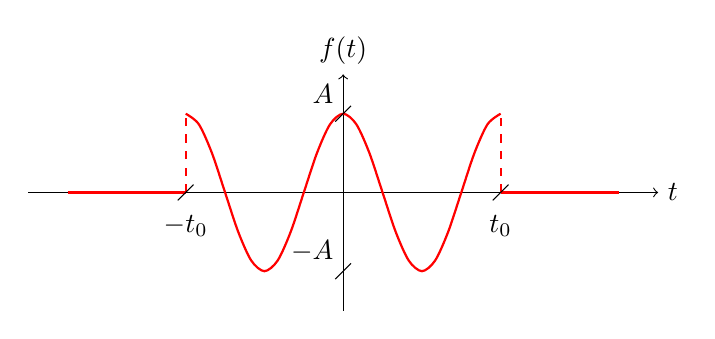
\begin{tikzpicture}
  %\draw (0,0) circle (1in);
  \draw[->] (-4.0,+0.0) -- (+4.0,+0.0) node[right] {$t$};
  \draw[->] (+0.0,-1.5) -- (+0.0,+1.5) node[above] {$f(t)$};
  \draw[-,red, thick] (-3.5,+0.0) -- (-2.0,0.0);
  \draw[-,red, thick] (+2.0,+0.0) -- (+3.5,0.0);
  \draw[scale=1.0,domain=-2.0:2.0,smooth,variable=\x,red,thick] plot ({\x},{1.0*cos(\x*180)});%96%3.141592
  \draw[-,red, thick, dashed] (+2.0,+0.0) -- (+2.0,1.0);
  \draw[-,red, thick, dashed] (-2.0,+0.0) -- (-2.0,1.0);
  
  
  \draw[-] (-2.0-0.1,-0.1)--(-2.0+0.1,0.1) node[midway, below, outer sep=5pt,align=center] {$-t_0$};
  \draw[-] (+2.0-0.1,-0.1)--(+2.0+0.1,0.1) node[midway, below, outer sep=5pt] {$t_0$};
  \draw[-] (-0.1,+1.0-0.1)--(+0.1,+1.0+0.1) node[midway, above left] {$A$};
  \draw[-] (-0.1,-1.0-0.1)--(+0.1,-1.0+0.1) node[midway, above left] {$-A$};
\end{tikzpicture}
\end{figure}

\begin{equation}
f(t)=\begin{cases}
0 & t \in \left( -\infty; -t_0 \right ) \\
A \cdot cos\left(\frac{2\pi}{t_0}\cdot t\right) & t \in \left( -t_0; t_0 \right ) \\
0 & t \in \left( t_0; \infty \right )
\end{cases} 
\end{equation}

\TT{Transformatę Fouriera obliczamy ze wzoru:}{The Fourier transform is defined as:}

\begin{equation}
F(\jmath \omega )=\int_{-\infty }^{\infty}f(t) \cdot e^{-\jmath \cdot \omega \cdot t}\cdot dt
\end{equation}

\TT{Podstawiamy do wzoru na transformatę wzór naszej funkcji:}{For the given $f(t)$ signal we get:}

\begin{align*}
F(\jmath \omega )&=\int_{-\infty }^{\infty}f(t) \cdot e^{-\jmath \cdot \omega \cdot t}\cdot dt=\\
&=\int_{-\infty }^{-t_0} 0 \cdot e^{-\jmath \cdot \omega \cdot t} \cdot dt + \int_{-t_0 }^{t_0} A \cdot cos\left(\frac{2\pi}{t_0}\cdot t\right) \cdot e^{-\jmath \cdot \omega \cdot t} \cdot dt + \int_{t_0 }^{\infty} 0 \cdot e^{-\jmath \cdot \omega \cdot t} \cdot dt =\\
&=\begin{Bmatrix}
cos(x) = \frac{e^{\jmath \cdot x}+e^{-\jmath \cdot x}}{2}
\end{Bmatrix}=\\
&=\int_{-\infty }^{-t_0} 0 \cdot dt + \int_{-t_0 }^{t_0} A \cdot \frac{e^{\jmath \cdot \frac{2\pi}{t_0}\cdot t}+e^{-\jmath \cdot \frac{2\pi}{t_0}\cdot t}}{2} \cdot e^{-\jmath \cdot \omega \cdot t} \cdot dt + \int_{t_0 }^{\infty} 0 \cdot dt =\\
&=0 + \frac{A}{2} \cdot \int_{-t_0 }^{t_0} \left(e^{\jmath \cdot \frac{2\pi}{t_0}\cdot t}+e^{-\jmath \cdot \frac{2\pi}{t_0}\cdot t}\right) \cdot e^{-\jmath \cdot \omega \cdot t} \cdot dt + 0 =\\
&=\frac{A}{2} \cdot \int_{-t_0 }^{t_0} \left(e^{\jmath \cdot \frac{2\pi}{t_0}\cdot t}\cdot e^{-\jmath \cdot \omega \cdot t}+e^{-\jmath \cdot \frac{2\pi}{t_0}\cdot t}\cdot e^{-\jmath \cdot \omega \cdot t}\right) \cdot dt =\\
&=\frac{A}{2} \cdot \int_{-t_0 }^{t_0} \left(e^{\jmath \cdot \frac{2\pi}{t_0}\cdot t -\jmath \cdot \omega \cdot t}+e^{-\jmath \cdot \frac{2\pi}{t_0}\cdot t -\jmath \cdot \omega \cdot t}\right) \cdot dt =\\
&=\frac{A}{2} \cdot \int_{-t_0 }^{t_0} \left(e^{\jmath \cdot \left(\frac{2\pi}{t_0} - \omega \right) \cdot t}+e^{-\jmath \cdot \left(\frac{2\pi}{t_0} + \omega \right) \cdot t}\right) \cdot dt =\\
&=\frac{A}{2} \cdot \left( \int_{-t_0 }^{t_0} e^{\jmath \cdot \left(\frac{2\pi}{t_0} - \omega \right) \cdot t} \cdot dt + \int_{-t_0 }^{t_0} e^{-\jmath \cdot \left(\frac{2\pi}{t_0} + \omega \right) \cdot t} \cdot dt \right)=\\
&=\begin{Bmatrix}
z_1=\jmath \cdot \left(\frac{2\pi}{t_0} - \omega \right) \cdot t & z_2=-\jmath \cdot \left(\frac{2\pi}{t_0} + \omega \right) \cdot t\\
dz_1=\jmath \cdot \left(\frac{2\pi}{t_0} - \omega \right) \cdot dt & dz_2=-\jmath \cdot \left(\frac{2\pi}{t_0} + \omega \right) \cdot dt\\
dt=\frac{1}{\jmath \cdot \left(\frac{2\pi}{t_0} - \omega \right)} \cdot dz_1 & dt=\frac{1}{-\jmath \cdot \left(\frac{2\pi}{t_0} + \omega \right)} \cdot dz_2\\
\end{Bmatrix}=\\
&=\frac{A}{2} \cdot \left( \int_{-t_0 }^{t_0} e^{z_1} \cdot \frac{1}{\jmath \cdot \left(\frac{2\pi}{t_0} - \omega \right)} \cdot dz_1  + \int_{-t_0 }^{t_0} e^{z_2} \cdot \frac{1}{-\jmath \cdot \left(\frac{2\pi}{t_0} + \omega \right)} \cdot dz_2 \right)=\\
&=\frac{A}{2} \cdot \left(  \frac{1}{\jmath \cdot \left(\frac{2\pi}{t_0} - \omega \right)} \cdot \int_{-t_0 }^{t_0} e^{z_1} \cdot dz_1  + \frac{1}{-\jmath \cdot \left(\frac{2\pi}{t_0} + \omega \right)} \cdot \int_{-t_0 }^{t_0} e^{z_2} \cdot  dz_2 \right)=\\
&=\frac{A}{2} \cdot \left(  \frac{1}{\jmath \cdot \left(\frac{2\pi}{t_0} - \omega \right)} \cdot \left. e^{z_1} \right|_{-t_0 }^{t_0}  + \frac{1}{-\jmath \cdot \left(\frac{2\pi}{t_0} + \omega \right)} \cdot \left. e^{z_2} \right|_{-t_0 }^{t_0} \right)=\\
&=\frac{A}{2} \cdot \left(  \frac{1}{\jmath \cdot \left(\frac{2\pi}{t_0} - \omega \right)} \cdot \left. e^{\jmath \cdot \left(\frac{2\pi}{t_0} - \omega \right) \cdot t } \right|_{-t_0 }^{t_0}  + \frac{1}{-\jmath \cdot \left(\frac{2\pi}{t_0} + \omega \right)} \cdot \left. e^{-\jmath \cdot \left(\frac{2\pi}{t_0} + \omega \right) \cdot t} \right|_{-t_0 }^{t_0} \right)=\\
&=\frac{A}{2} \cdot \left(  \frac{1}{\jmath \cdot \left(\frac{2\pi}{t_0} - \omega \right)} \cdot \left( e^{\jmath \cdot \left(\frac{2\pi}{t_0} - \omega \right) \cdot t_0 } - e^{\jmath \cdot \left(\frac{2\pi}{t_0} - \omega \right) \cdot (-t_0) } \right) \right. +\\ 
&+\left. \frac{1}{-\jmath \cdot \left(\frac{2\pi}{t_0} + \omega \right)} \cdot \left(e^{-\jmath \cdot \left(\frac{2\pi}{t_0} + \omega \right) \cdot t_0} - e^{-\jmath \cdot \left(\frac{2\pi}{t_0} + \omega \right) \cdot (-t_0)}\right) \right)=\\
&=\frac{A}{2} \cdot \left(  \frac{1}{\jmath \cdot \left(\frac{2\pi}{t_0} - \omega \right)} \cdot \left( e^{\jmath \cdot \left(\frac{2\pi}{t_0} - \omega \right) \cdot t_0 } - e^{-\jmath \cdot \left(\frac{2\pi}{t_0} - \omega \right) \cdot t_0 } \right) \right. +\\
&\left.+ \frac{1}{-\jmath \cdot \left(\frac{2\pi}{t_0} + \omega \right)} \cdot \left(e^{-\jmath \cdot \left(\frac{2\pi}{t_0} + \omega \right) \cdot t_0} - e^{\jmath \cdot \left(\frac{2\pi}{t_0} + \omega \right) \cdot t_0}\right) \right)=\\
&=\frac{A}{2} \cdot \left(  \frac{1}{\jmath \cdot \left(\frac{2\pi}{t_0} - \omega \right)} \cdot \left( e^{\jmath \cdot \left(\frac{2\pi}{t_0} - \omega \right) \cdot t_0 } - e^{-\jmath \cdot \left(\frac{2\pi}{t_0} - \omega \right) \cdot t_0 } \right) \right.+\\
&\left.+ \frac{1}{\jmath \cdot \left(\frac{2\pi}{t_0} + \omega \right)} \cdot \left(e^{\jmath \cdot \left(\frac{2\pi}{t_0} + \omega \right) \cdot t_0} - e^{-\jmath \cdot \left(\frac{2\pi}{t_0} + \omega \right) \cdot t_0}\right) \right)=\\
&=\frac{A}{2} \cdot \left(  \frac{1}{\jmath \cdot \left(\frac{2\pi}{t_0} - \omega \right)} \cdot \left( e^{\jmath \cdot \left(\frac{2\pi}{t_0} - \omega \right) \cdot t_0 } - e^{-\jmath \cdot \left(\frac{2\pi}{t_0} - \omega \right) \cdot t_0 } \right)\cdot \frac{2}{2} \right.+\\
&\left.+ \frac{1}{\jmath \cdot \left(\frac{2\pi}{t_0} + \omega \right)} \cdot \left(e^{\jmath \cdot \left(\frac{2\pi}{t_0} + \omega \right) \cdot t_0} - e^{-\jmath \cdot \left(\frac{2\pi}{t_0} + \omega \right) \cdot t_0}\right) \cdot \frac{2}{2} \right)=\\%#
&=\frac{A}{2} \cdot \left(  \frac{2}{\left(\frac{2\pi}{t_0} - \omega \right)} \cdot \frac{e^{\jmath \cdot \left(\frac{2\pi}{t_0} - \omega \right) \cdot t_0 } - e^{-\jmath \cdot \left(\frac{2\pi}{t_0} - \omega \right) \cdot t_0 } }{2 \cdot \jmath}  + \frac{2}{\left(\frac{2\pi}{t_0} + \omega \right)} \cdot \frac{e^{\jmath \cdot \left(\frac{2\pi}{t_0} + \omega \right) \cdot t_0} - e^{-\jmath \cdot \left(\frac{2\pi}{t_0} + \omega \right) \cdot t_0}}{2\cdot \jmath} \right)=\\
&=\begin{Bmatrix}
sin(x) = \frac{e^{\jmath \cdot x}-e^{-\jmath \cdot x}}{2\cdot \jmath}
\end{Bmatrix}=\\
&=\frac{A}{2} \cdot \left(  \frac{2}{\left(\frac{2\pi}{t_0} - \omega \right)} \cdot sin\left(\left(\frac{2\pi}{t_0} - \omega \right) \cdot t_0 \right)  + \frac{2}{\left(\frac{2\pi}{t_0} + \omega \right)} \cdot sin\left(\left(\frac{2\pi}{t_0} + \omega \right) \cdot t_0 \right) \right)=\\
&=\frac{A}{2} \cdot \left(  \frac{2}{\left(\frac{2\pi}{t_0} - \omega \right)} \cdot sin\left(\left(\frac{2\pi}{t_0} - \omega \right) \cdot t_0 \right)\cdot \frac{t_0}{t_0}  + \frac{2}{\left(\frac{2\pi}{t_0} + \omega \right)} \cdot sin\left(\left(\frac{2\pi}{t_0} + \omega \right) \cdot t_0 \right) \cdot \frac{t_0}{t_0}\right)=\\
&=\frac{A}{2} \cdot \left(  \frac{2\cdot t_0}{\left(\frac{2\pi}{t_0} - \omega \right)\cdot t_0} \cdot sin\left(\left(\frac{2\pi}{t_0} - \omega \right) \cdot t_0 \right)  + \frac{2 \cdot t_0}{\left(\frac{2\pi}{t_0} + \omega \right)\cdot t_0} \cdot sin\left(\left(\frac{2\pi}{t_0} + \omega \right) \cdot t_0 \right) \right)=\\
&=\frac{A}{2} \cdot \left(  2\cdot t_0 \cdot \frac{ sin\left(\left(\frac{2\pi}{t_0} - \omega \right) \cdot t_0 \right)}{\left(\frac{2\pi}{t_0} - \omega \right)\cdot t_0}  + 2 \cdot t_0 \cdot \frac{sin\left(\left(\frac{2\pi}{t_0} + \omega \right) \cdot t_0 \right)}{\left(\frac{2\pi}{t_0} + \omega \right)\cdot t_0} \right)=\\
&=\begin{Bmatrix}
Sa(x)=\frac{sin(x)}{x}
\end{Bmatrix}=\\
&=\frac{A}{2} \cdot \left(  2\cdot t_0 \cdot Sa\left(\left(\frac{2\pi}{t_0} - \omega \right) \cdot t_0 \right) + 2 \cdot t_0 \cdot Sa\left(\left(\frac{2\pi}{t_0} + \omega \right) \cdot t_0 \right) \right)=\\
&=A \cdot t_0 \cdot \left( Sa\left(\left(\frac{2\pi}{t_0} - \omega \right) \cdot t_0 \right) + Sa\left(\left(\frac{2\pi}{t_0} + \omega \right) \cdot t_0 \right) \right)
\end{align*}

\TT{Transformata sygnału $f(t)$ to $F(\jmath \omega)=A \cdot t_0 \cdot \left( Sa\left(\left(\frac{2\pi}{t_0} - \omega \right) \cdot t_0 \right) + Sa\left(\left(\frac{2\pi}{t_0} + \omega \right) \cdot t_0 \right) \right)$.}{The Fourier transform of the $f(t)$ is equal to $F(\jmath \omega)=A \cdot t_0 \cdot \left( Sa\left(\left(\frac{2\pi}{t_0} - \omega \right) \cdot t_0 \right) + Sa\left(\left(\frac{2\pi}{t_0} + \omega \right) \cdot t_0 \right) \right)$.}

\TT{Narysujmy widmo sygnału $f(t$ czyli:}{Draw complex spectrum of the $f(t)$:}

\begin{equation}
F(\jmath \omega)=A \cdot t_0 \cdot \left( Sa\left(\left(\frac{2\pi}{t_0} - \omega \right) \cdot t_0 \right) + Sa\left(\left(\frac{2\pi}{t_0} + \omega \right) \cdot t_0 \right) \right)
\end{equation}


\begin{figure}[H]
	\centering
	\begin{tikzpicture}
	\draw[->] (-5.0,+0.0) -- (+5.0,+0.0) node[right] {$\omega$};
	\draw[->] (+0.0,-2.5) -- (+0.0,+3.0) node[above] {$F(\jmath \cdot \omega)$};

	\draw[scale=1.0,domain=-4.0:4.0,samples=2000,smooth,variable=\x,red,thick] plot ({\x},{2*sinc((2-\x)*3.141592*2)+2*sinc((2+\x)*3.141592*2)});

	\draw[-] (-2.0-0.1,-0.1)--(-2.0+0.1,0.1) node[midway, below, outer sep=5pt] {-$\frac{2\pi}{t_0}$};

	\draw[-] (+2.0-0.1,-0.1)--(+2.0+0.1,0.1) node[midway, below, outer sep=5pt] {$\frac{2\pi}{t_0}$};

	\draw[-] (-0.1,+2.0-0.1)--(+0.1,+2.0+0.1) node[midway, above right] {$A \cdot t_0$};
    \draw[-] (-0.1,-2.0-0.1)--(+0.1,-2.0+0.1) node[midway, below right] {$-A\cdot t_0$};

	\end{tikzpicture}
\end{figure}

\TT{Widmo amplitudowe obliczamy ze wzoru:}{The magnitude spectrum is defined as:}

\begin{equation}
M(\omega)=\left | F(j \cdot \omega) \right |
\end{equation}

\begin{figure}[H]
	\centering
	\begin{tikzpicture}
	\draw[->] (-5.0,+0.0) -- (+5.0,+0.0) node[right] {$\omega$};
  \draw[->] (+0.0,-0.5) -- (+0.0,+3.0) node[above] {$F(\jmath \cdot \omega)$};
  
  \draw[scale=1.0,domain=-4.0:4.0,samples=2000,smooth,variable=\x,red,thick] plot ({\x},{abs(2*sinc((2-\x)*3.141592*2)+2*sinc((2+\x)*3.141592*2))});
  
  \draw[-] (-2.0-0.1,-0.1)--(-2.0+0.1,0.1) node[midway, below, outer sep=5pt] {-$\frac{2\pi}{t_0}$};
  \draw[-] (+2.0-0.1,-0.1)--(+2.0+0.1,0.1) node[midway, below, outer sep=5pt] {$\frac{2\pi}{t_0}$};
  \draw[-] (-0.1,+2.0-0.1)--(+0.1,+2.0+0.1) node[midway, above right] {$A \cdot t_0$};
  		
	\end{tikzpicture}
\end{figure}

\TT{Widmo aplitudowe sygnału rzeczywistego jest zawsze parzyste.}{The magnitude spectrum of a \underline{real signal} is an even-symmetric function of $k$.}

\TT{Widmo fazowe obliczamy ze wzoru:}{The phase spectrum is defined as:}

\begin{equation}
\Phi ( \omega )=\TT{arctg}{arctan2}\left(\frac{Im\{F(\jmath \cdot \omega )\}}{Re\{F(\jmath \cdot \omega )\}}\right)
\end{equation}

\begin{figure}[H]
	\centering
	\begin{tikzpicture}
	\draw[->] (-5.0,+0.0) -- (+5.0,+0.0) node[right] {$\omega$};
	\draw[->] (+0.0,-1.5) -- (+0.0,+2.0) node[above] {$\Phi(\omega)$};
	
	\draw[-,red] (-3.0,-1.0) -- (-2.5,-1.0);
	\draw[-,red] (-2.5,-0.0) -- (-1.5,-0.0);
	\draw[-,red] (-1.5,-1.0) -- (-1.0,-1.0);
	\draw[-,red] (-1.0,-0.0) -- (-0.5,-0.0);
    \draw[-,red] (-0.5,-1.0) -- (0.0,-1.0);
	\draw[-,red] (0.0,+1.0) -- (0.5,+1.0);
	\draw[-,red] (0.5,+0.0) -- (1.0,+0.0);
	\draw[-,red] (1.0,+1.0) -- (1.5,+1.0);
 	\draw[-,red] (1.5,+0.0) -- (2.5,+0.0);
    \draw[-,red] (2.5,+1.0) -- (3.0,+1.0);
	  
	\draw[-] (-1.0-0.1,-0.1)--(-1.0+0.1,0.1) node[midway, below, outer sep=5pt] {-$\frac{\pi}{t_0}$};
	\draw[-] (-2.0-0.1,-0.1)--(-2.0+0.1,0.1) node[midway, below, outer sep=5pt] {-$\frac{2 \pi}{t_0}$};
	\draw[-] (-3.0-0.1,-0.1)--(-3.0+0.1,0.1) node[midway, below, outer sep=5pt] {-$\frac{3 \pi}{t_0}$};
	\draw[-] (-4.0-0.1,-0.1)--(-4.0+0.1,0.1) node[midway, below, outer sep=5pt] {-$\frac{4 \pi}{t_0}$};
	\draw[-] (+1.0-0.1,-0.1)--(+1.0+0.1,0.1) node[midway, below, outer sep=5pt] {$\frac{\pi}{t_0}$};
	\draw[-] (+2.0-0.1,-0.1)--(+2.0+0.1,0.1) node[midway, below, outer sep=5pt] {$\frac{2 \pi}{t_0}$};
	\draw[-] (+3.0-0.1,-0.1)--(+3.0+0.1,0.1) node[midway, below, outer sep=5pt] {$\frac{3 \pi}{t_0}$};
	\draw[-] (+4.0-0.1,-0.1)--(+4.0+0.1,0.1) node[midway, below, outer sep=5pt] {$\frac{4 \pi}{t_0}$};
	\draw[-] (-0.1,+1.0-0.1)--(+0.1,+1.0+0.1) node[midway, left] {$\pi$};
	\draw[-] (-0.1,-1.0-0.1)--(+0.1,-1.0+0.1) node[midway, right] {-$\pi$};
	
	\end{tikzpicture}
\end{figure}

\TT{Widmo fazowe sygnału rzeczywistego jest zawsze nieparzyste.}{The phase spectrum of a \underline{real signal} is an odd-symmetric function of $k$.}

\end{task}

